\documentclass[twocolumn]{article}

\usepackage{graphicx}
\usepackage{enumitem}
\usepackage{hyperref}
\usepackage{float}

\title{Predicting Wine Quality and Acidity using Machine Learning and CRISP-DM
Methodology}
\author{César Cardoso, Rafael Pereira}
\date{\today}

\begin{document}
	\maketitle

	\begin{abstract}
		The quality of wine is a multifaceted characteristic influenced by various factors.
		This project employs machine learning techniques within the framework of the
		Cross-Industry Standard Process for Data Mining (CRISP-DM) methodology to
		predict wine quality ratings (1, 2, 3) and acidity levels. The study encompasses
		phases of business understanding, data exploration, preprocessing, modeling,
		evaluation, and deployment. Given the constraints of a small dataset, we opt
		for simpler models, specifically using Random Forest Classifier and Ridge Regression
		for classification and regression tasks, respectively. The dataset has been assumed
		to be clean, features have been standardized using the StandardScaler from
		scikit-learn, three random wines have been removed to facilitate a correct split
		during cross-validation with 5 folds, and models have been evaluated
		accordingly.
	\end{abstract}

	\section{Introduction}
	The world of viticulture produces a vast array of wines, each unique in flavor,
	aroma, and quality. Understanding and predicting wine quality is a complex challenge
	that can benefit from the application of machine learning. In addition to
	quality, we explore the prediction of wine acidity, a crucial parameter that
	influences the overall taste profile. This project leverages machine learning algorithms
	to predict both wine quality ratings (1, 2, 3) and acidity levels.

	\section{CRISP-DM Methodology}
	The Cross-Industry Standard Process for Data Mining (CRISP-DM) provides a structured
	framework for guiding data mining projects. Our application of CRISP-DM to the
	wine quality and acidity prediction project involves six key phases.

	\subsection{Business Understanding}
	In this initial phase, we aim to comprehend the business objectives and requirements
	surrounding the prediction of wine quality and acidity. Engaging with
	stakeholders and domain experts helps define the problem, establish success criteria,
	and set the stage for subsequent phases.

	\subsection{Data Understanding}
	Given the assumption of a clean dataset, the data understanding phase involves
	confirming the absence of data quality issues. We explore the dataset
	containing information on various wine characteristics, identify relevant features,
	and gain insights into potential challenges and opportunities. Additionally,
	three random wines were removed to facilitate a correct split during cross-validation
	with 5 folds.

	\begin{figure}[H] % Use H to force figure placement here
		\centering
		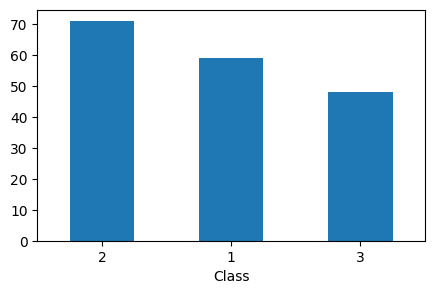
\includegraphics[width=1\linewidth]{winePerClass.png}
		\caption{Wine count per class}
		\label{fig:wine-count}
	\end{figure}

	\begin{figure}[H]
		\centering
		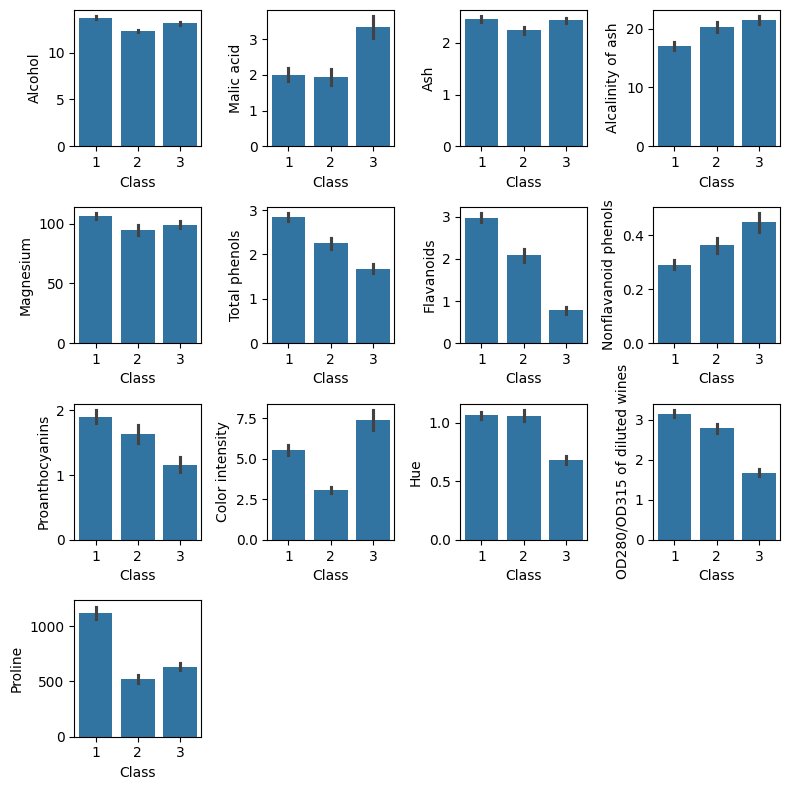
\includegraphics[width=1\linewidth]{Feature vs Class.png}
		\caption{Features related to each class}
		\label{fig:features-class}
	\end{figure}

	\begin{figure}[H]
		\centering
		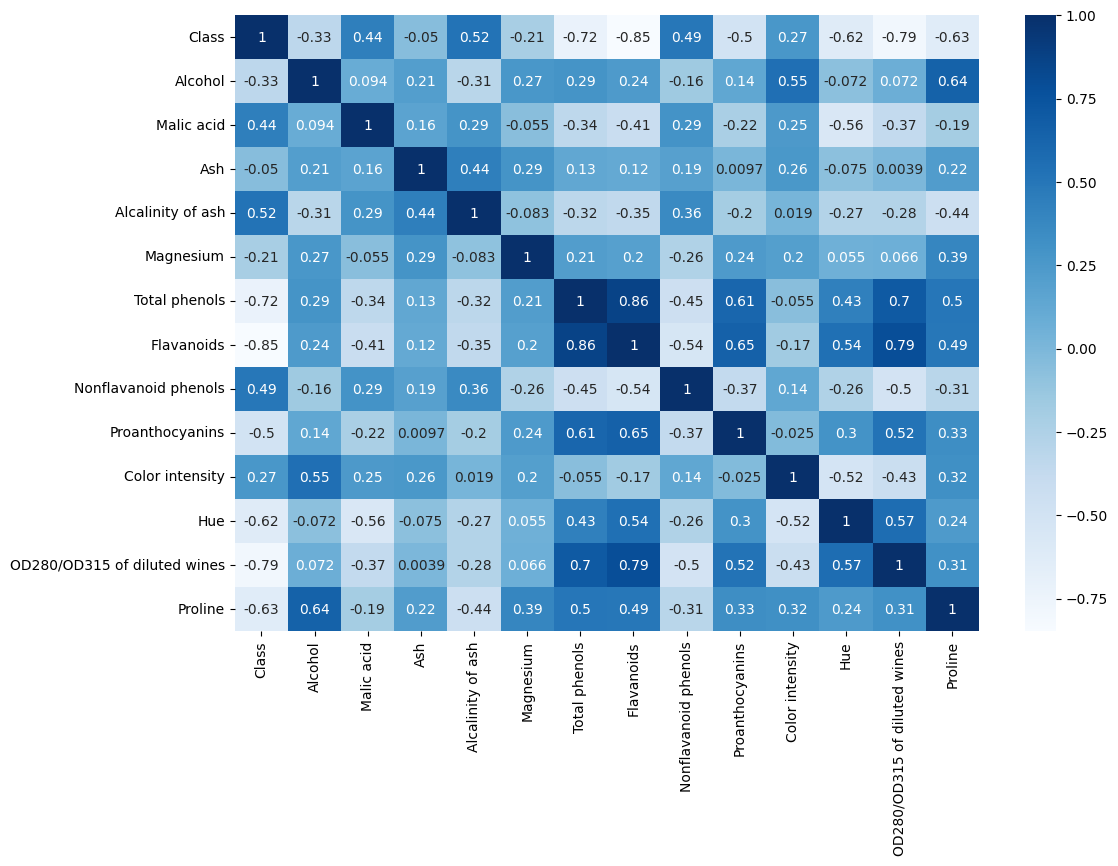
\includegraphics[width=1\linewidth]{Correlation.png}
		\caption{Correlation heatmap}
		\label{fig:correlation-heatmap}
	\end{figure}

	\begin{figure}[H]
		\centering
		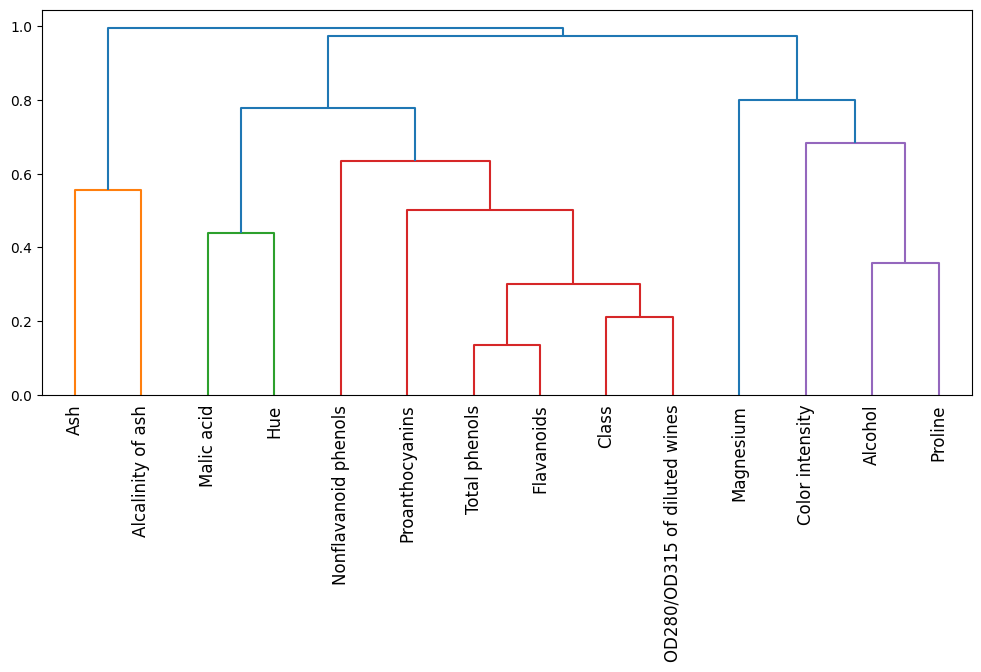
\includegraphics[width=1\linewidth]{Cluster Hierarchy.png}
		\caption{Clusters dendrogram (Hierarchical Clustering)}
		\label{fig:cluster-dendrogram}
	\end{figure}

	\begin{figure}[H]
		\centering
		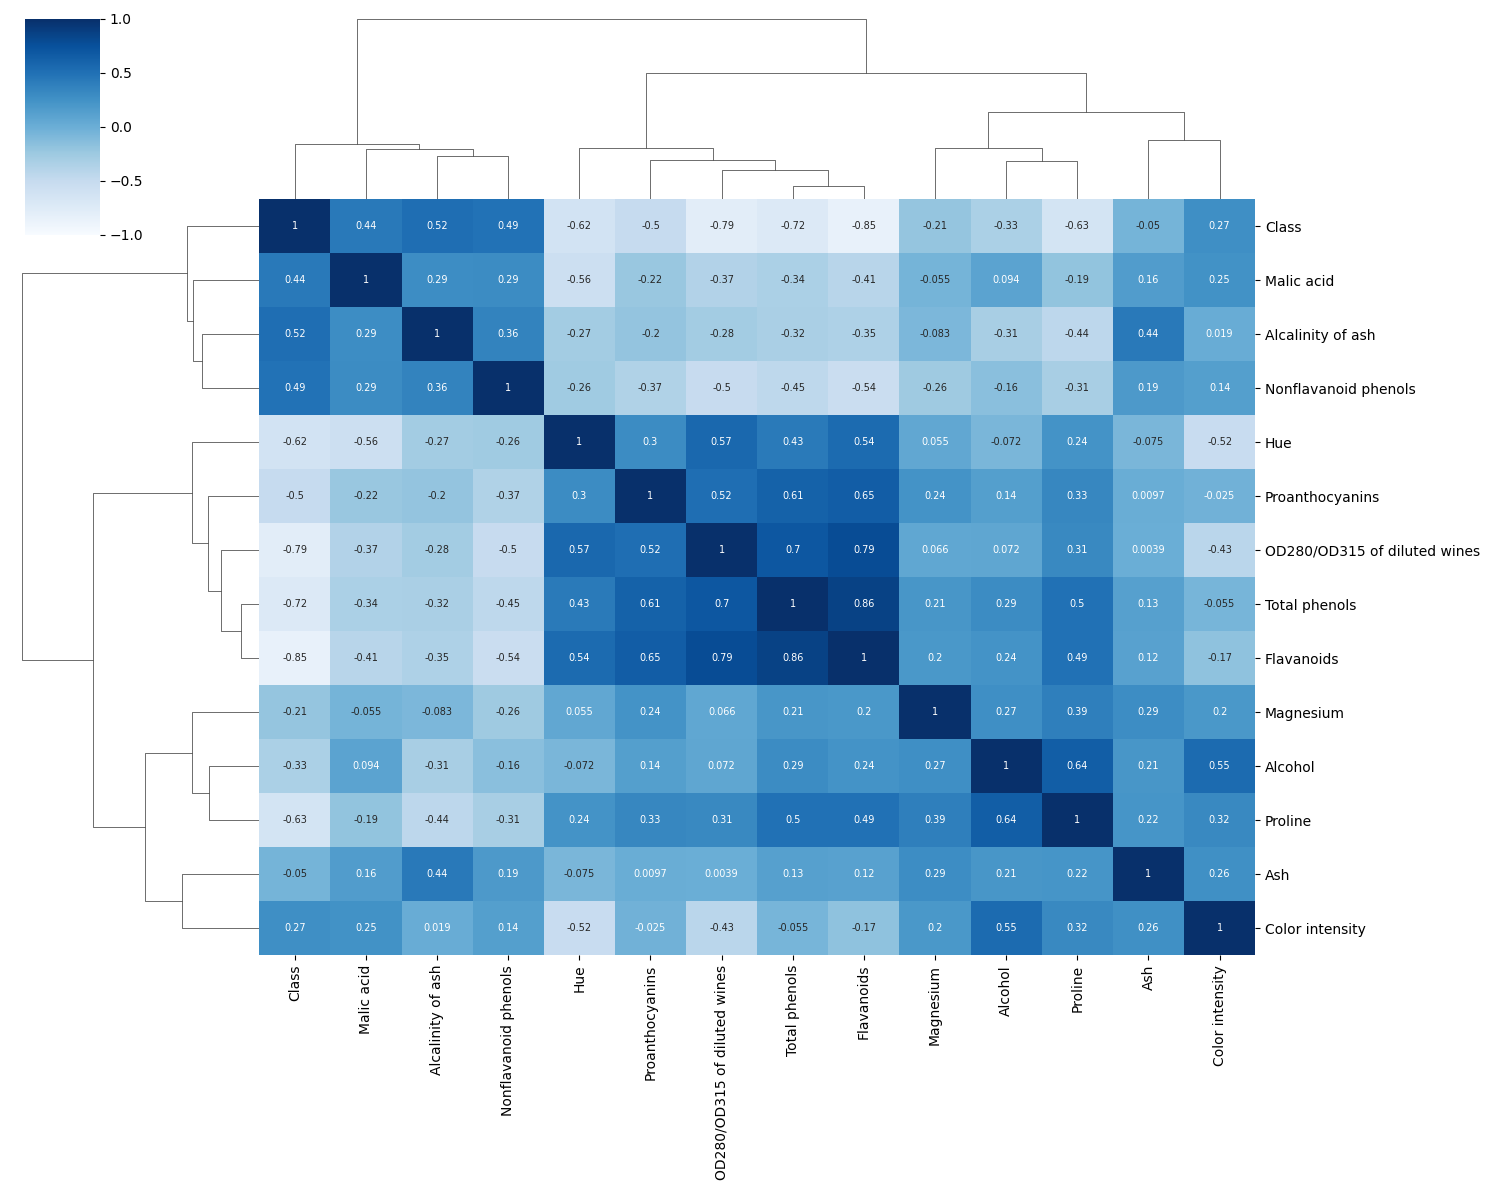
\includegraphics[width=1\linewidth]{Cluster Heatmap.png}
		\caption{Correlation heatmap with Clusters dendrogram}
		\label{fig:cluster-heatmap}
	\end{figure}

	\subsection{Data Preparation}
	With a clean dataset, the data preparation phase focuses on feature selection,
	normalization, and splitting into training and testing sets. To ensure standardized
	features, we use the StandardScaler from scikit-learn.

	\subsection{Modeling}
	The heart of the project lies in the modeling phase, where we employ simpler machine
	learning algorithms to accommodate the small dataset.

	\subsubsection{Classification for Wine Quality}
	For predicting wine quality ratings (1, 2, 3), we opt for Random Forest, an ensemble
	learning method suitable for handling small datasets with high accuracy. We
	employ StratifiedKFold with 5 folds for cross-validation, considering the removal
	of three random wines.

	\subsubsection{Regression for Wine Acidity}
	To predict wine acidity levels, we utilize Ridge Regression, a straightforward
	model suitable for regression tasks on small datasets with high correlation between features. A KFold with 5 folds is
	used for cross-validation, accounting for the removal of three random wines.

	\subsection{Evaluation}
	To assess the performance of our models, we employ various evaluation metrics,
	including accuracy, precision, recall, F1 score and AUC for classification, and
	Mean Squared Error (MSE), Root Mean Squared Error (RMSE), Mean Absolute Error(MAE),
	Normalized Mean Absolute Error (NMAE) and Root Squared ($R^{2}$) for regression.
	Cross-validation using StratifiedKFold(Classification) and Kfold(Regression)
	ensures the generalizability of our models to new and unseen data.

	\subsubsection{Evaluation Metrics and Formulas:}

	\begin{itemize}
		\item \textbf{Accuracy:}
			\[
				Accuracy = \frac{TP + TN}{TP + TN + FP + FN}
			\]

		\item \textbf{Precision:}
			\[
				Precision = \frac{TP}{TP + FP}
			\]

		\item \textbf{Recall (Sensitivity):}
			\[
				Recall = \frac{TP}{TP + FN}
			\]

		\item \textbf{F1 Score:}
			\[
				F1 Score = \frac{2 \times Precision \times Recall}{Precision + Recall}
			\]

		\item \textbf{Mean Squared Error (MSE):}
			\[
				MSE = \frac{1}{n}\sum_{i=1}^{n}(y_{i}- \hat{y}_{i})^{2}
			\]

		\item \textbf{Mean Absolute Error (MAE):}
			\[
				MAE = \frac{1}{n}\sum_{i=1}^{n}|y_{i}- \hat{y}_{i}|
			\]

		\item \textbf{Root Mean Squared Error (RMSE):}
			\[
				RMSE = \sqrt{\frac{1}{n}\sum_{i=1}^{n}(y_{i}- \hat{y}_{i})^{2}}
			\]

		\item \textbf{R-squared ($R^{2}$) Score:}
			\[
				R^{2}= 1 - \frac{\sum_{i=1}^{n}(y_{i}- \hat{y}_{i})^{2}}{\sum_{i=1}^{n}(y_{i}-
				\bar{y})^{2}}
			\]

		\item \textbf{Normalized Mean Absolute Error (NMAE):}
			\[
				NMAE = \frac{1}{Scale}\times \frac{\sum_{i=1}^{n}|y_{i}- \hat{y}_{i}|}{n}
			\]
	\end{itemize}

	\subsubsection{Model Performance and Results}
 
	\subsubsection{Random Forest Model Performance}
	The Random Forest model demonstrated high accuracy in predicting wine quality.
	The following are the detailed performance metrics:
    \smallskip

	\textbf{Overall Accuracy:} 0.9886 (98.86\%)
    \smallskip

	\textbf{Classification Report:}
	\begin{table}[H]
		\centering
		\begin{tabular}{|c|c|c|c|c|}
			\hline
			Class & Precision & Recall & F1-Score & Support \\
			\hline
			1     & 0.98      & 0.95   & 0.96     & 57      \\
			\hline
			2     & 0.96      & 0.97   & 0.97     & 71      \\
			\hline
			3     & 0.98      & 1.00   & 0.99     & 47      \\
			\hline
		\end{tabular}
		\caption{Classification report for the Random Forest model}
	\end{table}

	\textbf{Confusion Matrix:}
	\begin{table}[H]
		\centering
		\begin{tabular}{|c|c|c|c|}
			\hline
			         & Predicted 1 & Predicted 2 & Predicted 3 \\
			\hline
			Actual 1 & 54          & 3           & 0           \\
			\hline
			Actual 2 & 1           & 69          & 1           \\
			\hline
			Actual 3 & 0           & 0           & 47          \\
			\hline
		\end{tabular}
		\caption{Confusion matrix for the Random Forest model}
	\end{table}

	These results indicate the model's robustness in accurately classifying the
	wine quality into the three categories.

	\subsubsection{Logistic Regression Model Performance}

	The Logistic Regression model demonstrated excellent accuracy in predicting wine
	quality. Below are the detailed performance metrics:
\smallskip

	\textbf{Overall Accuracy:} 0.9771 (97.71\%)
\smallskip

	\textbf{Classification Report:}
	\begin{table}[H]
		\centering
		\begin{tabular}{|c|c|c|c|c|}
			\hline
			Class & Precision & Recall & F1-Score & Support \\
			\hline
			1     & 1.00      & 1.00   & 1.00     & 57      \\
			\hline
			2     & 0.99      & 0.97   & 0.98     & 71      \\
			\hline
			3     & 0.96      & 0.98   & 0.97     & 47      \\
			\hline
		\end{tabular}
		\caption{Classification report for the Logistic Regression model}
	\end{table}

	\textbf{Confusion Matrix:}
	\begin{table}[H]
		\centering
		\begin{tabular}{|c|c|c|c|}
			\hline
			         & Predicted 1 & Predicted 2 & Predicted 3 \\
			\hline
			Actual 1 & 57          & 0           & 0           \\
			\hline
			Actual 2 & 0           & 69          & 2           \\
			\hline
			Actual 3 & 0           & 1           & 46          \\
			\hline
		\end{tabular}
		\caption{Confusion matrix for the Logistic Regression model}
	\end{table}
	These results highlight the Logistic Regression model's capability in accurately
	classifying the wine quality into the three categories.
    \newpage
	\subsubsection{Comparing both models using receiver operating characteristic
	curves (ROC) and area under the curve (AUC)}

	\begin{figure}[H]
		\centering
		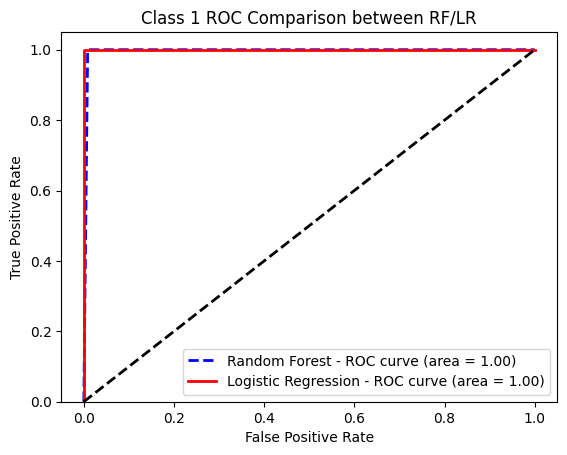
\includegraphics[width=1\linewidth]{ROC C1.png}
		\caption{Class 1 ROC}
		\label{fig:roc-c1}
	\end{figure}

	\begin{figure}[H]
		\centering
		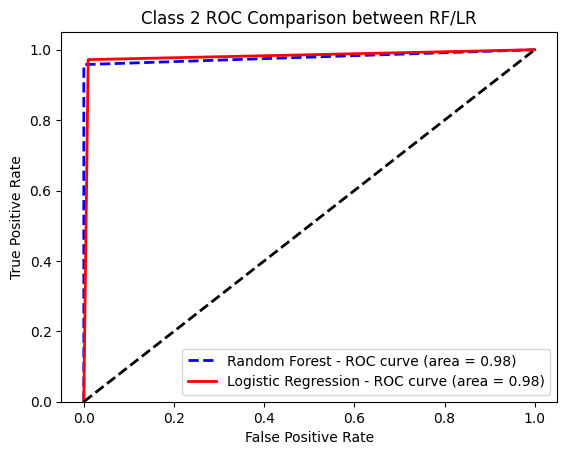
\includegraphics[width=1\linewidth]{ROC C2.png}
		\caption{Class 2 ROC}
		\label{fig:roc-c2}
	\end{figure}

	\begin{figure}[H]
		\centering
		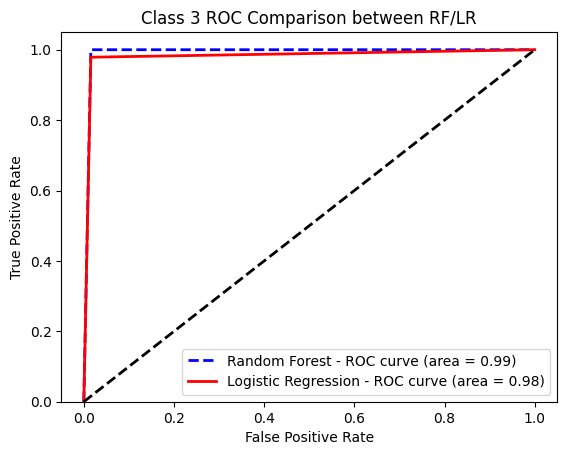
\includegraphics[width=1\linewidth]{ROC C3.png}
		\caption{Class 3 ROC}
		\label{fig:roc-c3}
	\end{figure}

	\subsubsection{Random Forest Regressor Model Performance}

	\[
		MSE = 0.878
	\]
	\[
		RMSE = 0.934
	\]
	\[
		MAE = 0.693
	\]
	\[
		NMAE = 0.291
	\]
	\[
		R^{2}= 0.311
	\]

	\begin{figure}[H]
		\centering
		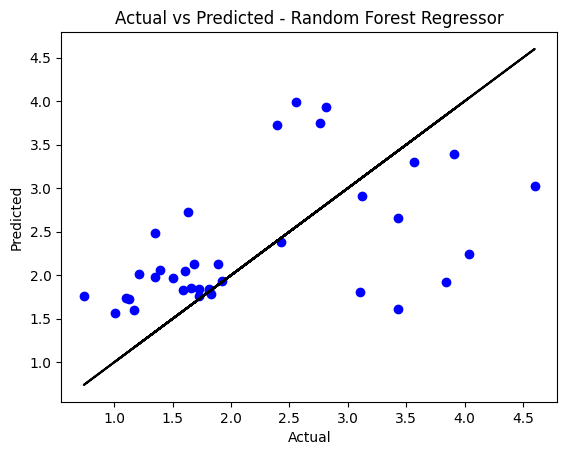
\includegraphics[width=.8\linewidth]{AvP RFR.png}
		\caption{Actual vs Predicted Malic Acid (Random Forest Regressor)}
	\end{figure}

	\subsubsection{Linear Regression Model Performance}

	\[
		MSE = 0.883
	\]
	\[
		RMSE = 0.937
	\]
	\[
		MAE = 0.721
	\]
	\[
		NMAE = 0.303
	\]
	\[
		R^{2}= 0.289
	\]

	\begin{figure}[H]
		\centering
		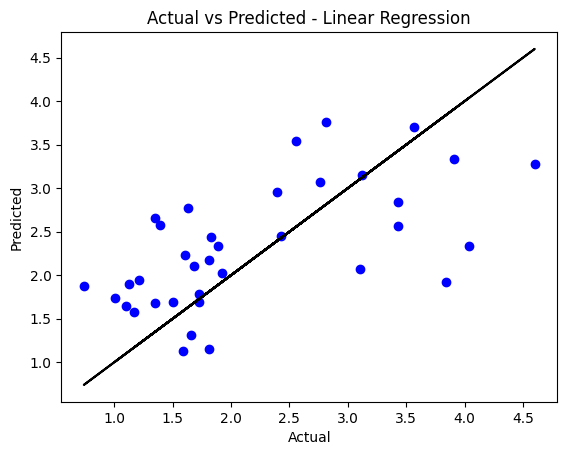
\includegraphics[width=.8\linewidth]{AvP LR.png}
		\caption{Actual vs Predicted Malic Acid (Linear Regressor)}
	\end{figure}
	\subsubsection{Ridge Regression Model Performance}
	\[
		MSE = 0.880
	\]
	\[
		RMSE = 0.936
	\]
	\[
		MAE = 0.717
	\]
	\[
		NMAE = 0.302
	\]
	\[
		R^{2}= 0.291
	\]
	\begin{figure}[H]
		\centering
		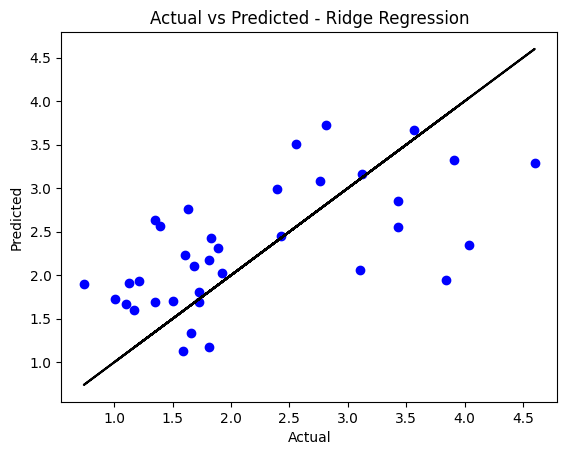
\includegraphics[width=.8\linewidth]{AvP RR.png}
		\caption{Actual vs Predicted Malic Acid (Ridge Regressor)}
	\end{figure}

	\subsection{Model Selection}
    Random Forest Classifier ended up being the preferred model to predict wine quality since it shows the highest average AUC in all the classes and the highest accuracy.\\
	To predict Malic Acid and given the high correlation among features in the dataset, Ridge Regression
	emerges as the best choice. It effectively handles multicollinearity with its L2
	regularization and demonstrates a balanced performance across key metrics.
	While RandomForestRegressor shows strong predictive accuracy and explanatory
	power, its complexity and interpretability are of concern. LinearRegression, though
	simpler, is less effective against multicollinearity.

	Ridge Regression offers a good balance between maintaining the simplicity of
	linear models and providing robustness against feature correlation. Its performance,
	with relatively low MSE, RMSE, and NMAE, along with a moderate R2 score,
	suggests effective predictive accuracy and a reasonable level of explanatory
	capability. Therefore, \textbf{Ridge Regression} is the most suitable model for
	this dataset, given its capability to provide reliable and interpretable
	results in the presence of high feature correlation.

	\subsection{Deployment}
	Upon selecting satisfactory models, we transition to the deployment phase.
	This involves integrating the models into a production environment, where they
	can make predictions on new wine data. Continuous monitoring and updates are
	essential to maintain the models' performance over time.

	\section{Conclusion}
	This document outlines a pragmatic approach to predicting wine quality and acidity
	using simpler machine learning models and the CRISP-DM methodology. Given the
	constraints of a small dataset, our focus on business understanding,
	streamlined data exploration, and the application of Random Forest Classifier and
	Ridge Regression in the modeling phase aims to develop interpretable and effective
	predictive models. The evaluation and deployment phases ensure the models' practical
	application in real-world scenarios.

	\section{References}
	\begin{enumerate}[label={[\arabic{*}]}]
		\item CRISP-DM. Cross-Industry Standard Process for Data Mining. \url{https://www.crisp-dm.org/}

		\item Scikit-learn: Machine Learning in Python. \url{https://scikit-learn.org/}

		\item Dealing with very small datasets.
			\url{https://www.kaggle.com/code/rafjaa/dealing-with-very-small-datasets/}

		\item Cortez, P., Cerdeira, A., Almeida, F., Matos, T., \& Reis, J. (2009).
			Modeling wine preferences by data mining from physicochemical properties. Decision
			Support Systems, 47(4), 547-553.

		\item Overcoming Issues with Small Data Sets when Building Machine Learning Models.
			\url{https://www.youtube.com/watch?v=Ly3ogCE-GuI&t=1638s}
	\end{enumerate}
\end{document}